

%%% This LaTeX source document can be used as the basis for your technical
%%% report. Intentionally stripped and simplified
%%% and commands should be adjusted for your particular paper - title, 
%%% author, citations, equations, etc.
% % Citations/references are in report.bib 

\documentclass[conference,backref=page]{acmsiggraph}

\TOGonlineid{45678}
\TOGvolume{0}
\TOGnumber{0}
\TOGarticleDOI{1111111.2222222}
\TOGprojectURL{}
\TOGvideoURL{}
\TOGdataURL{}
\TOGcodeURL{}

% Include this so that citations show up in blue and the page information is included in the reference section
\hypersetup{
    colorlinks = true, 
    linkcolor = blue,
    anchorcolor = red,
    citecolor = blue, 
    filecolor = red, 
}


\title{Travelling Salesman Problem - Algorithms and Data Structures Coursework}

\author{Ross Alan James McLaren \thanks{e-mail:40174116@live.napier.ac.uk} \\
Edinburgh Napier University\\
Algorithms and Data Structures (SET09117)}
\pdfauthor{Ross Alan James McLaren}

\begin{document}
\maketitle

\raggedbottom

\begin{abstract}

The travelling salesman problem is a difficult computational scenario to solve. At a very basic level the travelling salesman problem asks the following question: "Given a list of cities and the distances between each pair of cities, what is the shortest possible route that visits each city once and returns to starting city." When observing it from this basic view the problem seems very easy to solve and for very small numbers of cities this is true. However, the number of possible solutions is equal to (n-1)/2 where n equals the number of cities, knowing this we 
can determine that brute forcing the problem becomes impractical and eventually nearly impossible as the number of cities rise.

\end{abstract}



\keywordlist

%% Use this only if you're preparing a technical paper to be published in the 
%% ACM 'Transactions on Graphics' journal.

% \TOGlinkslist

% \copyrightspace


\section{Introduction}


\paragraph{The Problem}
The problem initially given is the design and implementation of an algorithm which will produce a solution to the travelling salesman problem. The problem should differ from the commonly known Nearest Neighbour solution either by being an edited, personal interpretation of the Nearest Neighbour algorithm or by using a completely different solution as a base.


\paragraph{Existing Solutions}
A common existing solution is the aforementioned Nearest Neighbour algorithm. This algorithm works by starting the salesman in the first city in the list and finding the closest city to the current city in the data set. Once this city has been found, the salesman's current city should be marked as visited and they should move to the next city. This should be repeated until every city in the list has been visited. This algorithm quickly yields a short tour, but it rarely produces the optimal one.
 
\begin{figure}[h]
	\centering
	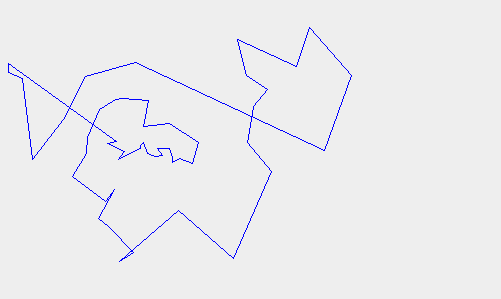
\includegraphics[width=1.0\columnwidth]{images/nearestNeighbourPath}
	\caption{Graphical representation of the Nearest Neighbour Algorithm using berlin52 data set.}
\end{figure}
    
\paragraph{Cities and Routes}
In the presented problem Cities are given as a list of geographical 2-D points. A route is devised by using an algorithm to sort the given list into the most efficient way(in terms of distance between points) to parse the list. If this is done optimally the algorithm will sort the list into the smallest route length in the shortest amount of time.

\paragraph{Solving the Problem}
The algorithm given in this report to solve TSP was developed over many iterations with each iteration taking the best elements of the previous and looking to improve upon the worst.

\paragraph{Proposed Solution}
The algorithm proposed in this report(which shall henceforth be known as the Nearest Three Neighbours Algorithm) is edited form of the Nearest Neighbour Algorithm. The results given by this algorithm differ from Nearest Neighbour in both route length and time taken.

\paragraph{Nearest Three Neighbours}
The Nearest Three Neighbours Algorithm follows the same basic principles of the Nearest Neighbour Algorithm - both find nearby cities to the current one, mark the current city as visited and move. A major difference is that instead of finding the closest city to the current, Nearest Three Neighbours finds the three closest. The next city in the route is chosen from these three at random - this follows the logic that it's acceptable to possibly take a longer route from one point to the next so long as it gives a shorter route overall. The Nearest Three Neighbours Algorithm also offers a random start point as well as looping through this process twenty times and taking the shortest route as the solution.

\begin{figure}[h]
	\centering
	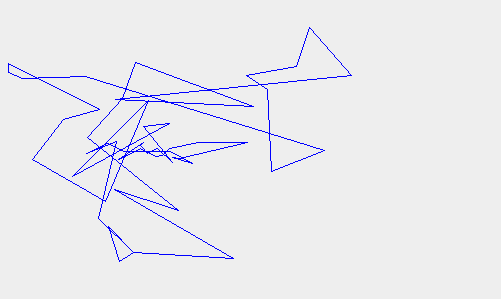
\includegraphics[width=1.0\columnwidth]{images/nearestThreeNeighboursPath}
	\caption{Graphical representation of the Nearest Three Neighbours Algorithm using berlin52 data set.}
\end{figure}

\paragraph{Limitations of Nearest Three Neighbours}
The Nearest Three Neighbours Algorithm does suffer from some limitations when compared to the standard Nearest Neighbour. One of these is the random elements present in the Nearest Three Neighbours Algorithm, because one of the three closest cities is chosen at random, it's very likely that a large amount of path crossing will occur - this is normally a loss in route length as the salesman would essentially be doubling back on himself to go to cities that he missed while travelling.  The Nearest Three Neighbours Algorithm also suffers more than Nearest Neighbour as the problem size increases as it is more computationally intensive - this generally causes it to also take more time to compute all problems. 


\section{Experimental Method} 

\paragraph{Algorithm Testing}
The solutions provided by the Nearest Three Neighbours Algorithm were tested via in-line testing to ensure that no cities were missed. This was done by comparing the input list of cities with the output list of results to ensure they were the same size. These sizes were printed out to be used in the compilation of results. A visual representation was also output, this was used to observe what sections of the route regularly overlap to allow for future refinements.

\paragraph{Algorithmic Comparisons}
As Nearest Neighbour is a well known algorithm capable of delivering good, although sub-optimal, results it was run first on the data sets in order to calculate a benchmark against which to test the Nearest Three Neighbours Algorithm.

\paragraph{Testing data} 
The sets of data used for testing were picked in order to demonstrate a range of sizes. Berlin52 was picked as it is a good demonstration for how quickly the problem can be solved with a relatively small number of cities(52). Both rl5915(containing 5915 cities) and rl5934(containing 5934 cities) were chosen to demonstrate the effect an extremely large data set has on the computation time. The data sets pr1002 and pcb3038, which contain 1002 and 3038 cities respectively, were chosen in order to accurately graph and visualise the rate of change for the time taken to compute.

\paragraph{Testing Process}
In order to compile valuable route lengths and computational times each data set was run five hundred times and had the average route length and computational time taken for the final result. This significantly lowers the risk of any external factor upsetting the results.

\section{Results}

\begin{table}[h]
	\resizebox{1.0\textwidth}{!}{
	\begin{minipage}{\textwidth}
	\centering
	\begin{tabular}{p{2.5cm}p{2.5cm}p{2.5cm}p{2.5cm}p{2.5cm}p{2.5cm}}
	Data Set & Average Nearest Neighbour Route & Average Nearest Neighbour Time(In ms) & Average Nearest Three Neighbours Route & Average Nearest Three Neighbours Time(In ms) & Number of Cities \\ [2ex]
	\hline
	berlin52 & 8980.92 & 0 & 15779.64 & 1 & 52 \\ [0.5ex]
	pr1002 & 315596.59 & 6 & 454033.15 & 66 & 1002 \\ [0.5ex]
	pcb3038 & 175572.75 & 48 & 406254.5 & 590 & 3038 \\ [0.5ex]
	rl5915 & 707498.63 & 179 & 2807782.86 & 2383 & 5915 \\ [0.5ex]
	rl5934 & 683805 & 182 & 2713385.83 & 2410 & 5934 \\ [0.5ex]
	
	\end{tabular}
		\caption[Table Caption Text]{Results collected from testing.}
		\label{Name of Table}
		\end{minipage}}
\end{table}
\clearpage

\begin{figure}[h]
	\centering
	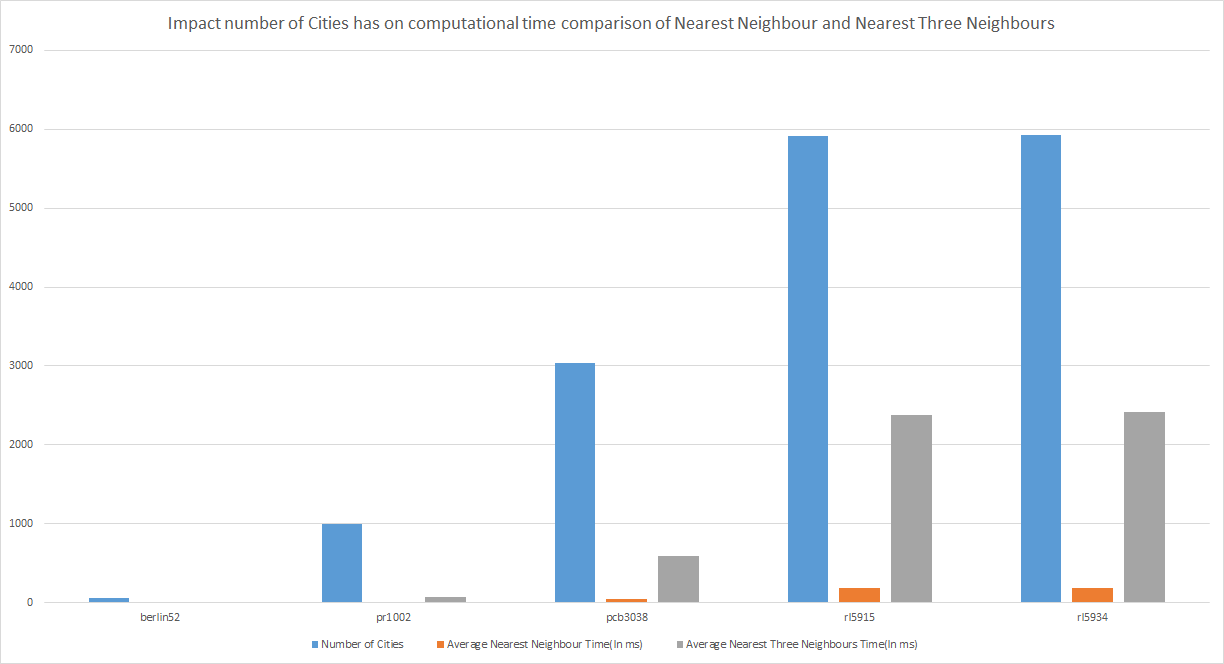
\includegraphics[width=0.75\textwidth]{images/barGraphOfCitiesImpactOnComputationalTime}
	\caption{Comparison of impact number of cities has on computational time for both Nearest Neighbour and Nearest Three Neighbours}
\end{figure}

\begin{figure}[h]
	\centering
	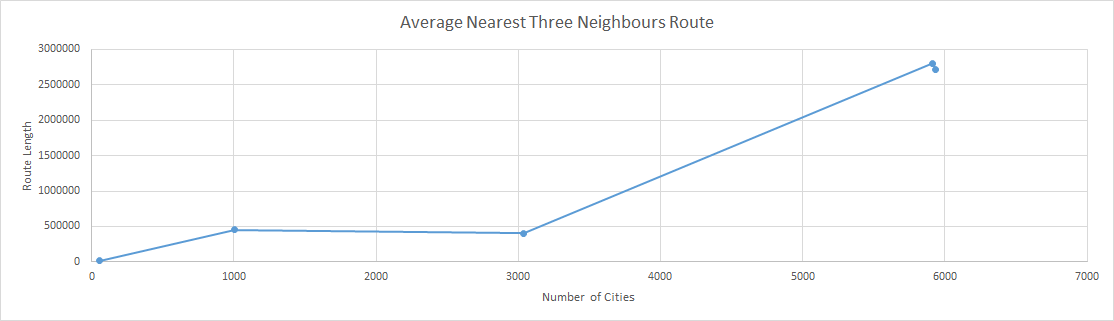
\includegraphics[width=0.75\textwidth]{images/effectOnRouteLengthByNumberOfCities}
	\caption{The impact that the number of cities has on the route length for Nearest Three Neighbours}
\end{figure}

% SIMULATION
\onecolumn
\twocolumn
\section{Simulation}

\paragraph{Overview}
You will start with a brief overview of the core principles and mechanism behind your effect.  This should be reflected in your final implementation, so consider what you will actually be implementing. What components make up the effect and how are they connected.

How does your simulation work and what are the reasons it is important.  This is a decisive section to put together as it will help you in the rest of your physics-based animation development.

\paragraph{Detailed description}
Provide a more detailed description of how the simulation functions. Consider the following aspects of the simulation:
\begin{itemize}
\item {\bf Functionality}: Describe what your simulation does and the anticipated boundaries of its functionality
\item {\bf Method}: Present the theory underpinning your technique (Mathematical, physics or algorithmic principles) and the technique itself. You should be able to articulate a general algorithm at this stage.
\item {\bf Control/interactivity}: Describe the interactive how the simulation will be controlled
\end{itemize}

\paragraph{Implementation}
At the design stage, you are not expected to provide information about the implementation, but you need to consider and reflect on the technical challenges that you will need to address. You also need to provide information about relevant technical aspects of your project. Please consider the following points:

\begin{itemize}
\item  {\bf Major Software Development Tasks} What are the major pieces of development to make the software work?  Identify the main tasks from the simulation design, particularly items you feel will be difficult to implement. 
\item {\bf Risks} What are the risks in your development?  Consider which pieces of functionality will be difficult to implement, and what are the options if you cannot achieve them.
\item {\bf External Libraries} Are you using any external libraries or resources to implement your simulation?  If you are using any libraries outside the ones developed in the practical sessions, these will need to be described here.
\end{itemize}

In your final report, this section will present the final implementation details. You should also reflect on the differences between the approach proposed in your design document and the final implementation.

% EVALUATION
\section{Testing and evaluation}
In this section of the {\bf Design document}, you should describe the tests that you are considering carrying out to test your evaluation and ensure that it works within its specified boundaries. In your {\bf Final report}, you will present the actual evaluation that you have carried out and reflect on its outcome. In particular, you may consider the actual performance of your simulation in relation to your initial goals. A comparison to relevant work would also be beneficial.

\section{Guidelines}
This section should be removed from your design report. Information provided here is to help you writing up your reports.


\section{Conclusion and Future work}
The report should finish with a summary to give a brief overview of what the reader should remember most.  What was most important? The future work part only needs to be covered in your final report.


% \section*{Acknowledgements}


\bibliographystyle{acmsiggraph}
\bibliography{report}

\end{document}

